\chapter{Introduzione a R e a RStudio}
\label{cap:introduzione}

% Circa 1h20m

\section*{Obiettivi di apprendimento}


\begin{multicols}{2}
\begin{tcolorbox}[width=1\linewidth, halign=left, colframe=blue!60, colback=white, boxsep=1mm, arc=3mm]

Domande

\begin{myitemize}
	\item Come interagire con R e RStudio?
	\item Come gestire l'ambiente R?
	\item Come istallare pacchetti R?
	\item Come chiedere aiuto?
\end{myitemize}

\end{tcolorbox} 
\columnbreak
\begin{tcolorbox}[width=1\linewidth, halign=left, colframe=blue!60, colback=white, boxsep=1mm, arc=3mm]

Obiettivi

\begin{myitemize}
	\item Descrivere lo scopo e lo scenario d'uso dei diversi pannelli in RStudio
	\item Usare R per operazioni aritmetiche e logiche 
	\item Definire una variabile e assegnarle un valore
	\item Usare funzioni
	\item Gestire lo spazio di lavoro
	\item Gestire i pacchetti
	\item Saper trovare informazioni sul funzionamento di una funzione
\end{myitemize}

\end{tcolorbox} 
\columnbreak
\end{multicols}


\section{RStudio}
\label{sec:RStudio}

La prima volta che si apre RStudio, dovreste vedere l'interfaccia con tre pannelli descritta in Figura~\ref{fig:rstudio}. Quando si apre un uno script R, si apre anche un pannello per modificarlo, che compare in alto nella colonna di sinistra, come mostrato in Figura~\ref{fig:rstudio-script}. Attenzione a non confondere i due pannelli di sinistra (la console interattiva con quello che consente la modifica degli script). Infatti, essi svolgono funzioni simili, ma molto diverse: la console permette di testare alcuni comandi, che verranno persi alla chiusura della sessione (quando chiudete RStudio), mentre l'editor consente di salvare i comandi che potranno essere eseguiti anche in seguito. 

\noindent Questa differenza ci permette di introdurre i due modi principali per interagire con RStudio:

\begin{myenumerate}
	\item fare dei test con la console interattiva e poi copiare i comandi che ci servono in uno script R. Questo \`e utile per piccoli test o per controllare che non ci siano errori (aka fare debug), ma diventa spesso laborioso e prono a errori (approccio sconsigliato)
	\item scrivere il proprio codice (comandi) nella finestra dell'editor e poi usare l'IDE per eseguirli. Questo permette di salvare il codice per usi futuri (approccio consigliato)
\end{myenumerate}

\noindent Non vi preoccupate se tutto questo ora sembra confuso, lo vedremo nella pratica nella Sezione~\ref{sec:Rscript}.

\begin{figure}[h]
 \centering
  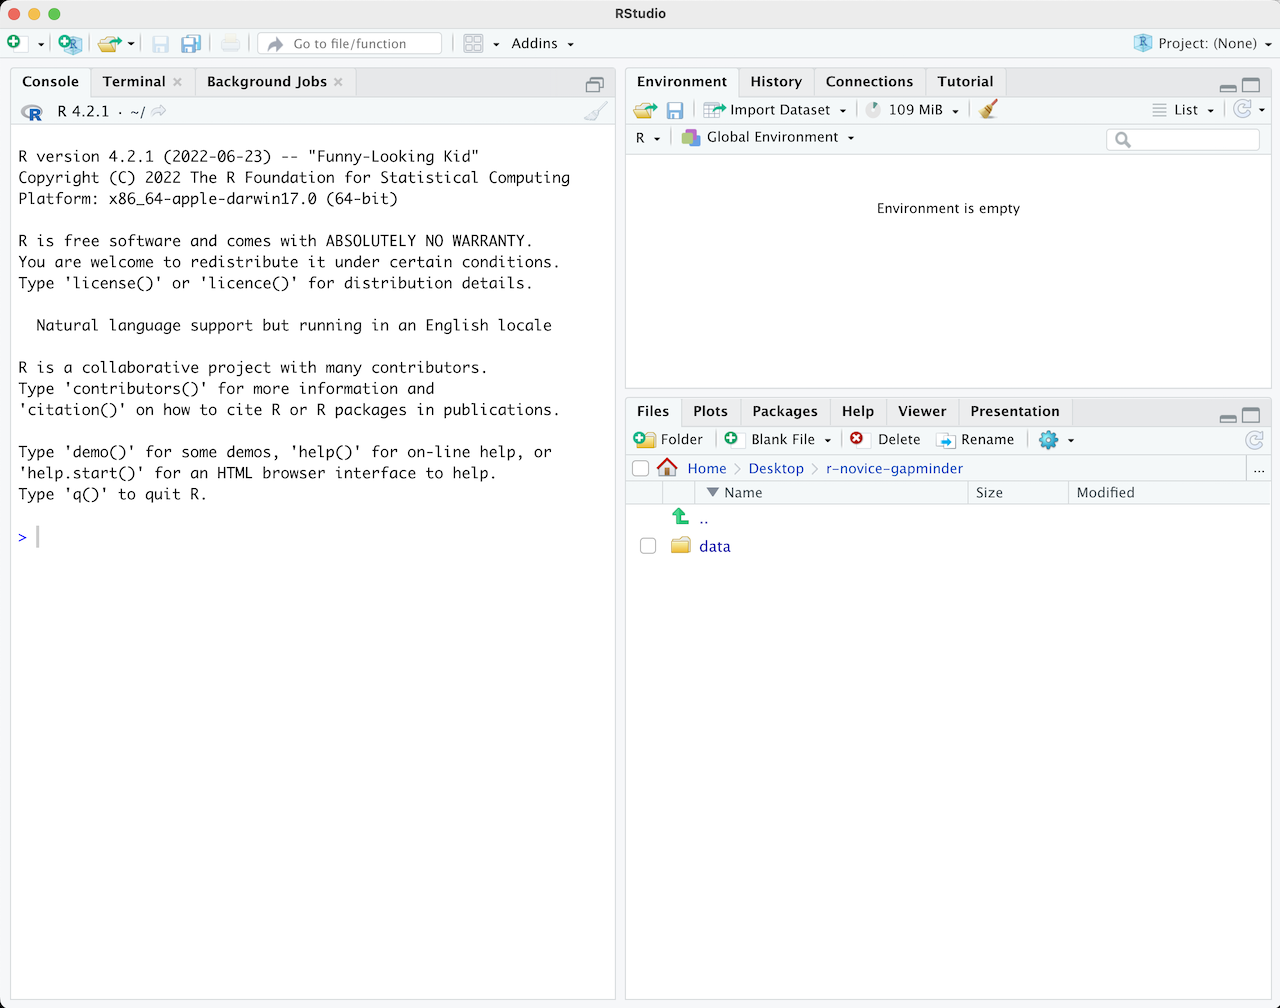
\includegraphics[width=0.7\textwidth]{images/01-rstudio.png}
  \label{fig:rstudio}
 \caption{L'interfaccia di RStudio con i tre pannelli che si vedono alla prima apertura del programma. La colonna di sinistra \`e interamente occupata dalla console (o terminale) interattivo, mentre la colonna di destra \`e divisa in due pannelli, in alto quello che elenca il contenuto dell'ambiente di lavoro e la storia dei comandi eseguiti, in basso quello che mostra il filesystem, i grafici che andremo a creare, e i messaggi di aiuto.}
\end{figure}


\begin{figure}[h!]
 \centering
  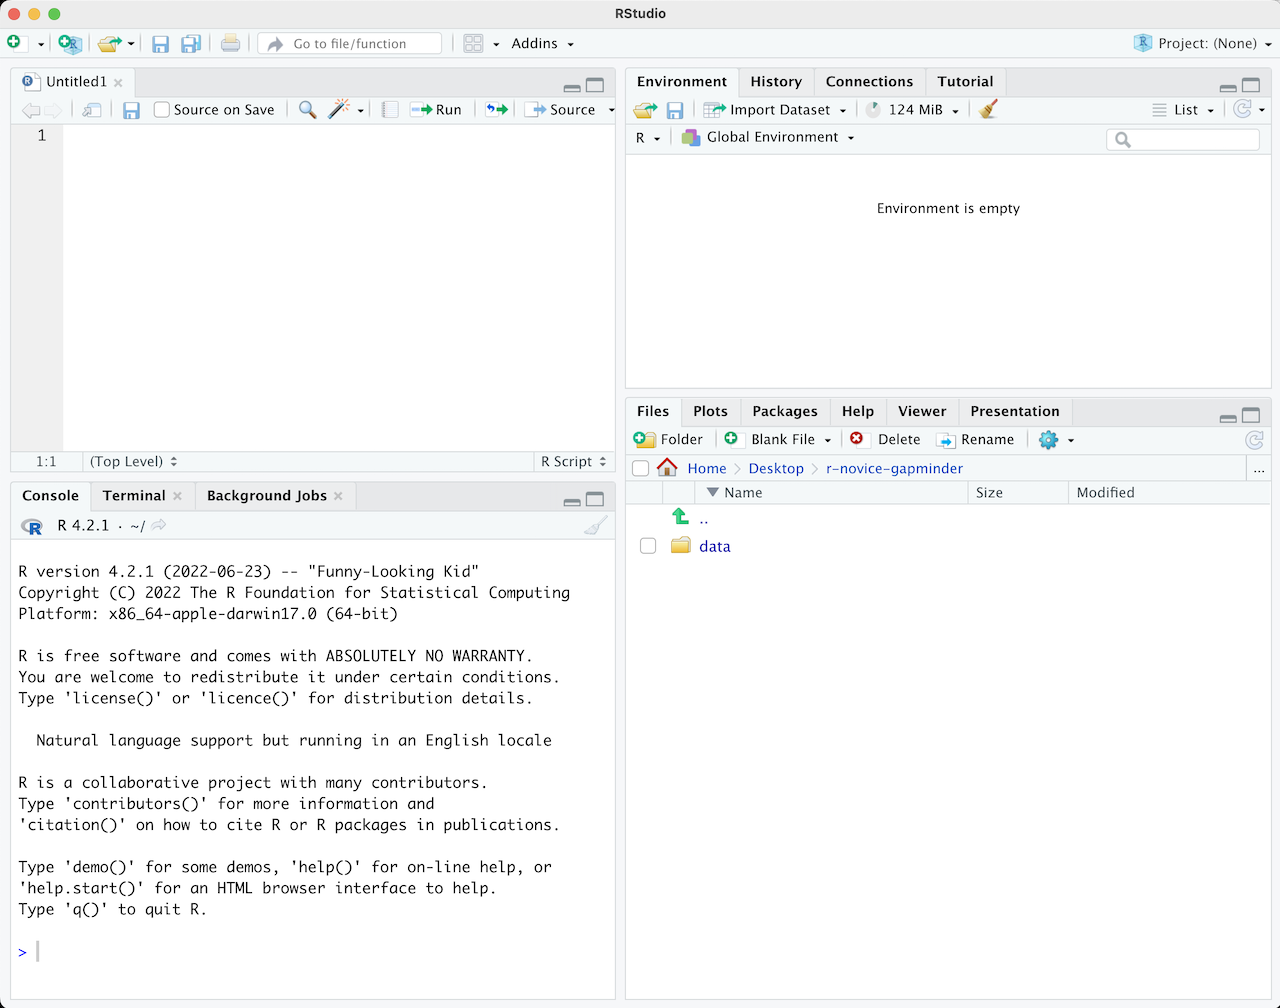
\includegraphics[width=0.7\textwidth]{images/01-rstudio-script.png}
   \label{fig:rstudio-script}
 \caption{L'interfaccia di RStudio con tutti e quattro i pannelli. Rispetto a Figure~\ref{fig:rstudio}, vediamo in alto a sinistra il pannello per la modifica degli script R. Il pannello con la console interattiva viene ridotto in basso a sinistra.}
\end{figure}


\section{Usare R come una calcolatrice}

La cosa pi\`u semplice che si pu\`o fare con R sono i calcoli aritmetici. Per esempio, se scrivete nella console:

\begin{lstlisting}[style=Rstyle]
1 + 100
\end{lstlisting}
%
e premete \lsin{Invio} (sulla tastiera) otterrete il seguente risultato

\begin{lstlisting}[style=Rstyle]
[1] 101
\end{lstlisting}
%
dove \lsin{[1]} rappresenta l'indice del primo elemento stampato in una linea della console (vedremo qualche esempio chiarificatore pi\`u aventi). 

\noindent
Se premete invio prima di completare un comando, R aspetter\`a che voi lo completiate. Per esempio, se scrivete

\begin{lstlisting}[style=Rstyle]
1 + 
\end{lstlisting}
%
e premete \lsin{Invio}, otterrete il seguente output

\begin{lstlisting}[style=Rstyle]
+ 
\end{lstlisting}
%
In generale, ogni volta che la sessione (riga nella console) mostra un \lsin{+} invece che un \lsin{>} vuol dire che R sta attendendo che voi completiate il comando -- se volete ritornare alla console, premete \lsin{ESC} sulla tastiera. Un'altra strategia \`e premere \lsin{Ctrl+C}. Questa seconda opzione vi permette anche di interrompere l'esecuzione di uno o pi\`u comandi, per esempio perch\'e sono molto (troppo) lunghi da eseguire o perch\'e  avete notato un errore nel codice. 


\subsection{L'ordine delle operazioni}

L'ordine in cui le operazioni aritmetiche sono svolte \`e quello classico, cio\`e (in ordine di precedenza):

\begin{myenumerate}
	\item parentesi: \lsin{()}
	\item esponenti: \lsin{^} oppure \lsin{**}
	\item moltiplicazioni: \lsin{*}
	\item divisioni: \lsin{/}
	\item addizioni: \lsin{+}
	\item sottrazioni: \lsin{-}
\end{myenumerate}	

\noindent Se scriviamo sulla console:

\begin{lstlisting}[style=Rstyle]
3 + 5 * 2
\end{lstlisting}
%
otteniamo:

\begin{lstlisting}[style=Rstyle]
[1] 13
\end{lstlisting}
%
Perci\`o, se l'ordine di esecuzione \`e diverso da quello di default, o anche sono per chiarezza, \`e meglio utilizzare le parentesi:

\begin{lstlisting}[style=Rstyle]
(3 + 5) * 2
\end{lstlisting}
%
otteniamo:
\begin{lstlisting}[style=Rstyle]
[1] 16
\end{lstlisting}
%
Attenzione al modo in cui scrivete le operazioni e usate le parentesi: il codice potrebbe diventare illeggibile sia per voi che per altri. Per esempio:

\begin{lstlisting}[style=Rstyle]
(3 + (5 * (2 ^ 2))) # difficile da leggere
3 + 5 * 2 ^ 2       # chiaro, se ci si ricorda le regole
3 + 5 * (2 ^ 2)     # chiaro anche se non ricordiamo le regole
\end{lstlisting}
%
sono equivalenti:
\begin{lstlisting}[style=Rstyle]
[1] 23
\end{lstlisting}

\subsection{I commenti nel codice}

L'hash (\lsin{#} indica l'inizio di un commento, ovvero una stringa che viene ignorata da R e serve al programmatore/analista per capire cosa il codice stia facendo. Qualsiasi cosa che venga scritta dopo un \lsin{#} viene ignorata da R.

\subsection{La notazione scientifica}

Numeri molto grandi (o molto piccoli) vengono trasformati in notazione scientifica:

\begin{lstlisting}[style=Rstyle]
2/100000
[1] 2e-05
\end{lstlisting}

\begin{lstlisting}[style=Rstyle]
2*100000
[1] 2e+05
\end{lstlisting}
%
dove \lsin{e-05} vuol dire moltiplica per $10^{-5}$. Quindi, \lsin{2e-05} vuol dire $2 \times 10^{-5}$ e  \lsin{2e+05} vuol dire $2 \times 10^{5}$.



\section{Funzioni matematiche (e non solo)}
\label{sec:Rfunctions}

R offre una serie di funzioni matematiche ma anche (e non solo) di sistema. Le funzioni si invocano digitando il loro nome, seguite da aperta chiusa parentesi tonda. Alcune funzioni prendono uno o pi\`u argomenti, che andremo a inserire all'interno delle parentesi, separati da virgole.


\noindent Per esempio:

\begin{lstlisting}[style=Rstyle]
sqrt(9) # radice quadrata
[1] 3
\end{lstlisting}
%
prende un argomento, il numero di cui vogliamo fare la radice quadrata.

\begin{lstlisting}[style=Rstyle]
round(33.333333, 1) # arrotondamento
[1] 33.3
\end{lstlisting}
%
prende due argomenti, il primo argomento \`e il numero che deve essere arrotondato in modo che abbia tante cifre decimali quanto specificato dal secondo argomento.

\begin{lstlisting}[style=Rstyle]
ls() # lista
\end{lstlisting}
%
non prende nessun argomento e ci stampa tutti gli oggetti che sono presenti nel nostro ambiente (lo vedremo pi\`u nel dettaglio in Sezione~\ref{sec:environment}).

\noindent Non vi preoccupate se non ricordate il nome di una funzione: Google \`e vostro amico, e se ne ricordate almeno l'inizio potete usare l'auto-completamento con il \lsin{TAB} (sulla tastiera).


\section{Chiedere aiuto}

In generale, se si digita \lsin{?} prima del nome di una funzione (per esempio: \lsin{?function_name}) si aprir\`a la sua pagina di aiuto nel pannello in basso a destra di RStudio. Un comando analogo \`e \lsin{help(function_name)}.

\begin{lstlisting}[style=Rstyle]
?round
\end{lstlisting}

\noindent La pagina di aiuto contiene una descrizione dettagliata del comando e dei suoi argomenti, seguito, spesso, da un esempio di codice che illustra come deve essere usato. In generale, queste sono le sezioni pi\`u utili che trovate nella pagina di aiuto: 

\begin{myitemize}
\item    \emph{Description:} una descrizione pi\`u o meno estesa di cosa faccia una funzione 
\item    \emph{Usage:} gli argomenti di una funzione, con eventuali parametri di default (che possono essere modificati) 
\item    \emph{Arguments: } informazioni pi\`u dettagliate sul tipo di dati che ciascun argomento si aspetta
\item    \emph{Details: } qualsiasi dettaglio che lo sviluppatore ha ritenuto utile evidenziare
\item    \emph{Value:} il tipo di dati restituito in output dalla funzione
\item    \emph{Examples:} esempi di uso della funzione. In RStudio, se li evidenziate e premete \lsin{Ctrl+Return} potete eseguirli nella console.
\end{myitemize}


\noindent Se non vi ricordate il nome esatto di una funzione potete usare l'operatore \lsin{??} per fare una ricerca approssimata. Per esempio, se vi ricordate che include la parola \lsin{set} potete usare:

\begin{lstlisting}[style=Rstyle]
??set
\end{lstlisting}
%
per visualizzare, nel pannello in basso a destra di RStudio, un elenco di funzioni che la contengano.


\section{Comparare oggetti}

\begin{lstlisting}[style=Rstyle]
1 == 1  # uguale a?
[1] TRUE
1 == 2  # uguale a?
[1] FALSE

1 != 1  # diverso da?
[1] FALSE
1 != 2  # diverso da?
[1] TRUE

1 < 2   # Minore di?
[1] TRUE

1 <= 1  # Minore o uguale a?
[1] TRUE

1 >= -2 # Maggiore o uguale a?
[1] TRUE
\end{lstlisting}


\subsection{Comparare variabili continue}

Il \emph{numeri a virgola mobile} sono il modo in cui un calcolatore rappresenta delle (approssimazioni) dei numeri reali. Visto che sono delle approssimazioni, alcune cose che ci paiono ovvie, diventano molto meno ovvie:


\begin{lstlisting}[style=Rstyle]
0.1 + 0.05 
[1] 0.15

0.1 + 0.05 == 0.15 
[1] FALSE
\end{lstlisting}
%
Per ovviare a questo problema, quando si vogliono comparare numeri a virgola mobile, si usa la funzione \lsin{all.equal}:

\begin{lstlisting}[style=Rstyle]
all.equal(0.1 + 0.05, 0.15)
[1] TRUE
\end{lstlisting}


\section{Variabili}

Per assegnare un valore a una variabile si possono usare due notazioni, la freccia (\lsin{<-}), che \`e lo standard in R, o il singolo simbolo di uguale (\lsin{=})\footnote{Attenzione a non confonderlo con il doppio simbolo di uguale \lsin{==} che viene usato per comparare due oggetti.}:

\begin{lstlisting}[style=Rstyle]
x <- 1
y = 1
\end{lstlisting}
%
Notiamo che l'operazione di assegnazione non stampa nulla a video. Per visualizzare il valore di una variabile dobbiamo scriverne il nome a terminale:

\begin{lstlisting}[style=Rstyle]
x
[1] 1
y
[1] 1
\end{lstlisting}

\noindent
Se guardate nel pannello in alto a destra di RStudio, vedrete che una variabile \lsin{x} e una \lsin{y} sono apparse insieme al loro valore.

\vspace{0.2cm}

\noindent
Le variabili possono essere usate in vece dei valori che rappresentano:

\begin{lstlisting}[style=Rstyle]
z <- 9

sqrt(z)
[1] 3

sqrt(z) + 1
[1] 4
\end{lstlisting}
%
Le variabili possono anche essere riassegnate, sia con nuovi valori sia con i valori contenuti da altre variabili sia con i risultati di operazioni tra variabili:

\begin{lstlisting}[style=Rstyle]
x <- 4
y <- x
z <- sqrt(y) + x

x
[1] 4
y
[1] 4
z
[1] 6
\end{lstlisting}

\noindent In R\footnote{Altri linguaggi di programmazione possono seguire regole diverse.}, il nome di una variabile non pu\`o mai iniziare con un numero o con un underscore (\lsin{_}) n\'e contenere spazi o trattini (\lsin{-}). Variabili che iniziano con un punto, sono variabili ``nascoste''. 

\begin{mybox}{Variabile (informatica)}
In informatica, il termine variabile indica un ``contenitore'' un cui sono contenuti dei valori che possono o meno essere modificati durante l'esecuzione di un programma.

La variabile \`e definita da un ``nome'', ovvero una sequenza di lettere o numeri. \`E consigliabile che il nome della variabile rappresenti il suo contenuto, per esempio, \lsin{weight, height, BMI}. In caso di nomi lunghi, ci sono diverse strategie: 
\lsin{periods.between.words} (considerato il classico in R),
\lsin{underscores_between_words} (pi\`u leggibile), e
\lsin{camelCaseToSeparateWords} (meno leggibile).

Attenzione a non confondere variabili (il contenitore) con i valori (il contenuto).
\end{mybox}


\vspace{0.5cm} 

\begin{exercise}\label{ex2.1}

\noindent
Quali dei seguenti nomi di variabile sono validi in R?

\begin{lstlisting}[style=Rstyle]
min_height
max.height
_age
.mass
MaxLength
min-length
2widths
celsius2kelvin
\end{lstlisting}

	\exnote{Suggerimenti}%
	\begin{myitemize}
		\item provate a assegnare loro un valore 
	\end{myitemize}
\end{exercise}


\vspace{0.5cm} 

\begin{exercise}\label{ex2.2}

\noindent
Quale sar\`a il valore delle variabili \lsin{x} e \lsin{y} dopo che il seguente codice \`e stato eseguito?

\begin{lstlisting}[style=Rstyle]
x <- 50.5
y <- 122
x <- x * 2
y <- y - 20
\end{lstlisting}
	
\end{exercise}	


\vspace{0.5cm} 

\begin{exercise}\label{ex2.3}

\noindent
Scrivi un comando per capire se \lsin{x} sia pi\`u grande di \lsin{y}.

\end{exercise}	


\section{Gestire l'ambiente R}
\label{sec:environment}

Ci sono alcuni comandi molto utili per interagire con l'ambiente R.

\begin{lstlisting}[style=Rstyle]
ls()
[1] "x" "y" "z"
\end{lstlisting}
%
elenca (in ordine alfanumerico) tutte le variabili e funzioni che sono caricate nella vostra sessione di lavoro (o \emph{global environment})
%
Attenzione alle variabili nascoste, ovvero quelle che iniziano per \lsin{.}: per elencarle dovrete usare la funzione \lsin{ls} con il parametro \lsin{all.names=TRUE}

\begin{lstlisting}[style=Rstyle]
.hidden <- "nascosta"

ls()
[1] "x" "y" "z"

ls(all.names=TRUE)
[1] ".hidden" "x" "y" "z"
\end{lstlisting}
%
Quando assegniamo il valore a un parametro (l'argomento di una funzione, vedi sezione~\ref{sec:Rfunctions}) dobbiamo usare l'operatore \lsin{=}. Se si usa \lsin{<-} ci potrebbero essere dei side effects, o, pi\`u probabilmente un messaggio di errore:

\begin{lstlisting}[style=Rstyle]
ls(all.names <- TRUE)
(*@\textbf{\textcolor{red}{ Error in as.environment(pos) : invalid object for 'as.environment' }}@*)
\end{lstlisting}

\begin{mybox}{Warnings vs Errors}
	
Un errore indica che R non pu\`o proseguire con la computazione. Warnings, invece, indicano che la funzione \`e stata eseguita, ma probabilmente non ha funzionato come previsto. In entrambi i casi, R stampa a video un messaggio che dovrebbe aiutarvi a capire cosa \`e successo (o da copiare e incollare su Google, per quello che \`e importante installare R in inglese). In entrambi i casi, R vi segnala che c'\`e un problema che non dovreste ignorare.

\end{mybox}


\noindent Un altro comando utile per gestire con l'ambiente R \`e \lsin{rm()}, che elimina una o pi\`u variabili dall'ambiente di lavoro:

\begin{lstlisting}[style=Rstyle]
ls()
[1] "x" "y" "z"

rm(x)

ls()
[1] "y" "z"
\end{lstlisting}
%
Se avete molte variabili e le volete eliminare tutte, potete passare il loro elenco, come generato da \lsin{ls()} come parametro di \lsin{rm()}:

\begin{lstlisting}[style=Rstyle]
ls()
[1] "y" "z"

rm(list = ls())

ls()
character(0)
\end{lstlisting}
%
Attenzione: non potete pi\`u ripristinare una variabile eliminata. Come con i diamanti, un \lsin{rm} \`e per sempre.


\noindent Se quando chiamate una funzione vi dimenticate di aggiungere le parentesi dopo il nome, R stampa a video il codice della funzione stessa

\begin{lstlisting}[style=Rstyle]
rm

function (..., list = character(), pos = -1, envir = as.environment(pos), 
    inherits = FALSE) 
{
    if (...length()) {
        dots <- match.call(expand.dots = FALSE)$...
        if (!all(vapply(dots, function(x) is.symbol(x) || is.character(x), 
            NA, USE.NAMES = FALSE))) 
            stop("... must contain names or character strings")
        list <- .Primitive("c")(list, vapply(dots, as.character, 
            ""))
    }
    .Internal(remove(list, envir, inherits))
}
<bytecode: 0x1265d4d60>
<environment: namespace:base>
\end{lstlisting}
%
Perch\'e lo fa? Per R, chiamare qualcosa per nome indica la volont\`a dell'utente di stamparne il contenuto a video, sia questa una variabile numerica, una stringa di caratteri o una funzione.


\vspace{0.5cm} 

\begin{exercise}\label{ex2.4}

\noindent
Scrivi i comandi per creare due variabili \lsin{mass} e \lsin{age}, assegnare loro i valori 2.2 e 15, e poi rimuoverli dall'ambiente di lavoro.

\end{exercise}	

\noindent Sapere in che cartella ci troviamo \`e importante perch\`e quando dobbiamo accedere ad altri file (per esempio caricare dei dati, come vedremo in Sezione~\ref{sec:data_loading}) R andr\`a a cercarli in relazione alla cartella corrente.

\begin{lstlisting}[style=Rstyle]
# Visualizza la cartella corrente
getwd()
[1] "/Users/visconti/"

# Seleziona la cartella di lavoro
setwd("~/Desktop")

# Visualizza la cartella corrente
getwd()
[1] "/Users/visconti/Desktop/"
\end{lstlisting}

\begin{mybox}{Il filesystem}	

Il filesystem \`e la parte di un Sistema Operativo che \`e responsabile della gestione di file e cartelle. I file sono oggetti che contengono informazioni (testo, immagini, video, musica, programmi, \dots), e le cartelle sono oggetti che contengono file e/o altre cartelle. 

\noindent Le cartelle permettono di organizzare il contenuto del nostro computer in modo gerarchico, attraverso una struttura ad albero. Si parte dalla cartella principale detta ROOT (radice, indicata per esempio con \lsin{C:\} o \lsin{/} in Linux/Mac OS X), che contiene file e cartelle di secondo livello, che a loro volta conterranno altri file e cartelle di terzo livello e cos\`i via, in una serie di livelli annidati uno dentro l’altro.

\noindent La posizione di un file o di una cartella nel filesystem, e di conseguenza il percorso che bisogna fare per raggiungerli, pu\`o essere assoluto o relativo. Il percorso assoluto parte dalla cartella root. Il percorso relativo parte dalla cartella in cui ci troviamo (relativamente a essa per l'appunto) e sale o scende lungo l'albero delle cartelle.

\end{mybox}


\section{Pacchetti R}
\label{sec:R_package}

R \`e molto versatile perch\'e esistono moltissimi pacchetti (insiemi di funzioni, anche chiamate \emph{librerie}) che ci permettono di fare le cose pi\`u disparate.

\noindent I comandi R per gestire i pacchetti sono:

\begin{myitemize}
	\item \lsin{installed.packages()} visualizza i pacchetti installati
	\item \lsin{install.packages("packagename")} installa un pacchetto (attenzione alle virgolette doppie)
	\item \lsin{update.packages()} aggiorna i pacchetti installati
	\item \lsin{remove.packages("packagename")} disinstalla un pacchetto (attenzione alle virgolette doppie)
\end{myitemize}

\noindent Per poter usare un pacchetto (che sia stato precedentemente installato) serve caricarlo ad ogni sessione o all'inizio dello script che lo usa usando il comando \lsin{library(packagename)}.



\vspace{0.5cm} 

\begin{exercise}\label{ex2.5}

\noindent Installare il pacchetto R \lsin{ggplot2} utilizzando il seguente comando: 

\begin{lstlisting}[style=Rstyle]
install.packages("ggplot2", dependencies = TRUE)
\end{lstlisting}
%
Che comando usiamo per caricarlo nella sessione di lavoro?

\noindent Installate ora il pacchetto \lsin{ggrepel}.

\end{exercise}	


\vspace{0.5cm}

\begin{tcolorbox}[width=1\linewidth, halign=left, colframe=blue!60, colback=white, boxsep=1mm, arc=3mm]

\textbf{Punti principali}

\begin{myitemize}
    \item Usare  R per semplici operazioni aritmetiche e logiche
    \item Usare \lsin{<-} per assegnare un valore a una variabile
    \item Usare \lsin{ls()} per elencare le variabili in un ambiente di lavoro 
    \item Usare \lsin{rm()} per rimuovere una o pi\`u variabili dall'ambiente di lavoro 
    \item Usare \lsin{install.packages()} per installare un pacchetto R
	\item Usare \lsin{?, ?? o help()} per chiedere aiuto 
\end{myitemize}

\end{tcolorbox} 

